% Chapter 2

\chapter{Foundations and related work} % Chapter title

\label{ch:foundations} 

%----------------------------------------------------------------------------------------

Research on sentiment analysis has been vast and there are excellent summaries (cf. \cite{sentiment_analysis_summary_pang}, \cite{sentiment_analysis_summary_liu}, \cite{sentiment_analysis_association_metrics}). In the following, we will focus on work related to emotion detection, emotion verbs, and identifying the holder and the cause of an emotion. To avoid ambiguity, we will henceforth define sentiment as being positive or negative, while an emotion possesses more complex dimensions.

\section{Compositionality}

Sentiment and emotion are clearly compositional phenomenons. Sentiment clearly adheres to Montague's underlying \textit{principle of compositionality} and the notion of sentiment compositionality has been successfully applied in state-of-the-art approaches such as recursive neural tensor networks \cite{deep_sentiment_analysis}, which conceive the overall sentiment as a sum of the constituent polarities. However, compositionality for emotions is less clear: Two unemotive terms can -- combined -- evoke an emotion, e.g. \textit{stock falls}, \textit{the blind sees}. The emotion of this compound expression, though, cannot be calculated merely as the sum of its parts and can only be accurately predicted by making sense of the underlying world knowledge.

\citeauthor{adjective_noun_pairs} for instance construct a visual sentiment ontology containing more than 3,000 adjective-noun pairs (ANP). They obtain tags from Flickr and Youtube videos that are associated with any of Plutchik's emotions, rank them based on frequency, and determine their sentiment. This way, they retrieve 1,187 nouns (576 positive/negative, 611 neutral) and 268 positive and negative adjectives. They pair the adjectives and nouns to obtain ANPs such as \textit{beautiful flower} or \textit{disgusting food}. They are able to calculate the sentiment of the compound expression simply by summing the sentiment values of the adjective and the noun, assigning a higher weight to the adjective in case of opposite sentiment values to account for ANPs like \textit{abused child}. As emotion does not lend itself to easy compositionality, they have to fall back on additional information taken from Flickr meta-data to determine the emotion of the ANP.

\section{Emotive events}

Evidently, predicting emotion for events is harder than for nominal phrases, as modifiers contain a lot of meaningful information. As the above authors realized, adjectives like \textit{abused}, \textit{disgusting}, \textit{happy}, etc. almost always propagate their respective emotion to the whole nominal phrase.

\citeauthor{benefactive_malefactive} try to capture implicit attitudes by annotating benefactive/malefactive events, i.e. events that negatively or positively affect entities. Two annotators annotate a total of 725 sentences. They report 0.69 as overlapping agreement between event spans and good agreement (0.87 and 0.97) for agents and objects. Their annotation scheme, however, raises some doubts, as some neutral events are labeled as benefactive/malefactive, e.g. in \textit{She bakes a cake}, \textit{cake} is the object of the benefactive event.

\citeauthor{mutual_action} leverage world knowledge to detect emotions on an event level. Whereas we use association metrics derived from emotive contexts, their main insight is that the \textit{common mutual actions} between two event participants are a major cue for detecting emotions. For instance, a snake in general performs undesirable actions towards a girl, which would give the event \textit{a girl sees a snake} a negative emotion.

Given an event, they also account for active and passive. However, they don't match the patterns against an existing corpus as we do, but mine data from the web to generate mutual action histograms. They compare these to the histograms of a set of manually emotion-labelled events between reference pairs and return the emotion of the most similar histogram. They evaluate their system on 600 events manually labelled by ten annotators with a positive, negative, or neutral sentiment, omitting finer granularity. Their proposed emotion detection system achieves an accuracy of 81.0\% on events where a majority of 6 annotators agreed.

\section{Pattern-based mining for emotion detection} \label{sec:web-mining}

Similarly, \citeauthor{harvesting_ontologizing} leverage the web to automatically extract instances using patterns. Their method starts off with a set of seed instances, from which they induce and then select new patterns. In contrast to most unsupervised approaches, they not only use \emph{reliable} patterns (high precision, low recall), but also leverage generic patterns. They mitigate their imprecision by measuring pattern reliability based on instantiations of reliable patterns, which enables them to separate correct from incorrect instances. They evaluate their system on seven relations and show that without generic patterns, their system outperforms comparable systems in precision, while generic patterns improve its recall significantly, e.g. from a relative recall of 1.00 to 6.66 for the \textsc{is-a} relation in the CHEM corpus, while precision decreases from 85.0\% to 76.0\%.

While their approach is helpful for gathering knowledge to ontologize \texttt{is-a} and \texttt{part-of} relationships, the use of generic patterns for emotion detecion, which is already highly ambiguous, might introduce more noise and consequently rather hurt than improve performance. Furthermore, the difficulty of finding seed instances that will generate reliable patterns is amplified for emotions: \textit{I :: spiders}, \textit{I :: darkness},  \textit{I :: violence}, and \textit{I :: Bin Laden} might be promising seed instance to induce the pattern \textit{X hate Y}, they could also as easily be associated with \textit{X am scared of Y}, \textit{X object to Y}, etc; that is, while it is relatively straightforward to distil the essence of an \texttt{is-a} relationship via a set of seed instances, doing this for emotions is less easy and will invariably introduce a selection bias. Insofar, starting with a set of seed patterns and expanding them would be the preferred approach for emotion detection. We will leave this for future work.

\citeauthor{emotion_verbs} in turn use search query patterns to rank verb classes. They manually construct classes corresponding to the emotions surprise, fear, and annoyance and rank them by intensity of emotion by mining the lexical-semantic patterns \textit{X (perhaps) even Y}, \textit{X, not to say Y}, and \textit{If not X then Y} from the web. Their results indicate that some verbs such as \textit{intimidate}, \textit{scare}, and \textit{alarm}, while being similar, are not members of the same broader \textit{frighten} class. Example \ref{ex:emotion_verbs} shows their ordering of \textit{surprise} verbs.

\begin{align}
\begin{split}\label{ex:emotion_verbs}
&\textnormal{astonish > surprise > amaze > astound > strike > stun > floor}\\
&\textnormal{> dumbfound > flabbergast > stupefy}
\end{split}
\end{align}

While seed instances and patterns can be emotionally ambiguous, the micro-blogging platform Twitter provides a more salient indicator of emotions: hashtags. \citeauthor{twitter_hashtags_nrc} and \citeauthor{twitter_hashtags_bootstrapping} both use hashtags to extract emotion-evoking tweets. The former use emotions as hashtags, e.g. \textit{\#anger}, \textit{\#joy}, etc. to construct a Twitter emotion corpus by extracting 21,000 tweets containing these hashtags at the end of the message from the Twitter Search API\footnote{https://dev.twitter.com/rest/public/search}, with the joy emotion being prevalent in their corpus. They use an ensemble of binary SVM classifiers to predict the emotion hashtag of a tweet, achieving an F-score of 49.9 across all emotions, with disgust achieving the lowest (18.7) and joy the highest (62.4) scores.

The latter use a bootstrapping approach to learn new hashtags and hashtag patterns and harvest emotion phrases from these. They start by collecting 323,000 tweets containing seed hashtags like \textit{\#loveyou}, \textit{\#sweetheart}, and \textit{\#bff} for five emotions. They train a logistic regression classifier for each emotion, using tweets containing the seed hashtags as positive instances, with negative instances consisting of randomly selected tweets from a pool of unlabelled tweets. Applying the classifier to the pool of unlabelled tweets produces new emotion-labelled tweets, from which they retrieve the ten highest scoring emotion-indicating hashtags by computing the average probability assigned by the classifier. They also learn hashtag pattern (e.g. \textit{\#missedyoutoomuch} $\rightarrow$ \textit{\#missedyou*}) and emotion phrases (e.g. \textit{\#lovemylife} $\rightarrow$ \textit{love my life}) by representing hashtags in a trie data structure, applying the classifier to tweets matching the patterns and phrases, and selecting the ten patterns and phrases with the highest average probability respectively. They achieve the best performance (51-66 F-score across emotions) on a manually annotated corpus of 5,500 tweets with a hybrid approach of an SVM with n-gram features enhanced with the phrase-based classifier and the classifiers of their learned hashtags and hashtag patterns.

\section{Semantic roles in the context of emotions}

In the context of emotions, not only the nature of the emotional state, but also the person experiencing the emotion or the cause of the emotion are relevant. Semantic role labeling is the task in NLP that aims to identify these semantic arguments of the predicate and classify them into their specific roles. FrameNet \cite{framenet}, a linguistic resource that stores semantic role information in so-called frames related to certain contexts, lists the roles depicted in \ref{tab:core-roles-framenet} as core roles for its \textsc{emotions} frame.

\begin{table}[]
\centering
\begin{tabular}{ll}
{\bf Role}  & {\bf Description}                                                                                        \\
Event       & The occasion or happening that Experiencers in a\\
            & certain emotional state participate in.\\
Experiencer & The person or sentient entity that experiences or feels\\
            & the emotions.                                     \\
Expressor   & The body part, gesture, or other expression of the \\
            & Experiencer that reflects his or her emotional state. \\
State       & The abstract noun that describes a more lasting\\
            & experience by the Experiencer.                           \\
Stimulus    & The person, event, or state of affairs that evokes the\\
            & emotional response in the Experiencer.            \\
Topic       & The general area in which the emotion occurs. It\\
            & indicates a range of possible Stimulus.                
\end{tabular}
\caption{Core semantic roles in FrameNet's \textsc{emotion} frame.}
\label{tab:core-roles-framenet}
\end{table}

\citeauthor{emotion_holder} construct two models to identify the experiencer or holder of an emotion. The baseline model leverages the \textit{subject} dependency of emotional sentences, while an unsupervised syntax-based depends on the argument structure of emotional verbs. They acquire the argument structure in two ways: 
\begin{inparaenum}[(a)] [\itshape a\upshape)] \item from the dependency-parsed and \item from the part-of-speech tagged and chunked sentences. \end{inparaenum} They compare the sentence argument structure against frame syntaxes of 942 emotional verbs extracted from VerbNet, another linguistic resource. They report an F-Score of 64.83\% for the baseline and of 66.98\% and 62.39\% for the syntax-based model with argument structures acquired using dependencies and parts-of-speech respectively.

\citeauthor{semantic_role_labeling_tweets} frame the task of identifying the Experiencer, State, and Stimulus of an emotion as a classification task. They train their classifier on a dataset of 2012 US presidential election tweets with annotations crowd-sourced to Amazon's Mechanical Turk \footnote{https://www.mturk.com/mturk/welcome} and report an accuracy of 56.84 for detecting emotions and an F-score of 58.30 for detecting the stimulus. As their tweets deal with a narrowly defined domain, they are able to select the stimulus from a set of pre-chosen entities, which works for this narrow domain, but fails given an open set of potential stimuli.

\citeauthor{implicit_emotions} in contrast don't use IE techniques but base their approach on their knowledge base EmotiNet. As their knowledge base is focused on the family domain, they only consider that domain, where their approach outperforms an SVM algorithm trained on more data. They also remark that world knowledge is particularly valuable in cases where no emotion-bearing word, e.g. \textit{happy} is present.

\section{Typologies of emotion classification}

Psychologists have proposed a number of different theories for classifying emotions, e.g. distinguishing between instinctual and cognitive emotions. As emotions are inherently subjective, none has been universally accepted. Two classification theories have been frequently used by the research community: Ekman's and Plutchik's. \citeauthor{ekman_basic_emotions} proposes a theory with six basic emotions: anger, disgust, fear, joy, sadness, and surprise. According to \citeauthor{plutchik}, there are two additional ones: anticipation and trust. He depicts them in a wheel, shown in figure \ref{fig:plutchik}, where the intensity of the emotion increases with the proximity to the center, and organizes them in four opposing pairs: joy--sadness, trust--disgust, fear--anger, surprise--anticipation.

\begin{figure}[bth]
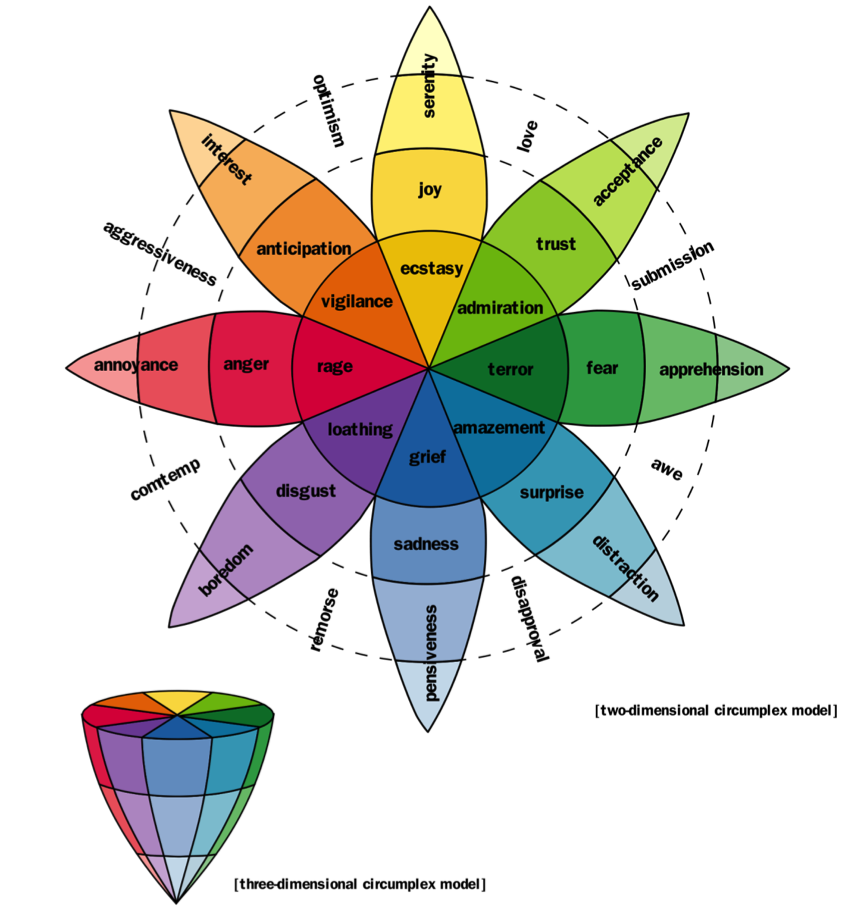
\includegraphics[width=.80\linewidth]{gfx/plutchik_wheel_emotion.png}
\caption{Plutchik's emotion wheel}\label{fig:plutchik}
\end{figure}

We adopted Plutchik's emotion classification for the following reasons: \begin{inparaenum}[(a)] [\itshape a\upshape)] \item it is clearly founded in psychological research; \item it is a superset of Ekman's six basic emotions; and \item its use by other researchers (cf. \cite{nrc}, \cite{adjective_noun_pairs}, \cite{emotions_novels_fairy_tales}) increases the comparability and transferability of our work.
\end{inparaenum}

\section{Sentiment and emotion lexica}

Sentiment lexica have been pervasive in sentiment analysis. Their use has a long history. The General Inquirer \cite{general_inquirer}, the first sentiment lexicon to our knowledge, was created in 1961. It contains 11,788 words labeled with 182 categories of word tags, some of which are relevant to emotions: It contains 1045 positive words, with a subset tagged for indicating affiliation or supportiveness. It contains 1160 negative words, a subset of which is tagged for indicating an attitude or concern with hostility or aggressiveness. 168 words are tagged with \textsc{pleasure} indicating the enjoyment of a feeling; 254 \textsc{pain} words indicate suffering, lack of confidence, or commitment; 49 \textsc{feel} words describe particular feelings, including gratitude, apathy, and optimism; 166 \textsc{arousal} words indicate excitation (aside from pleasures or pains); finally 311 \textsc{emot} words relate to different emotions such as \textit{admiration}, \textit{annoyance}, etc. It was key in early experiments such as differentiating fake suicide notes from real ones, among others. Since then, it has been used for a plethora of other applications, particularly sentiment analysis, e.g. for contextualizing polarity \cite{general_inquirer_usage}. 

WordNet-Affect \cite{wordnet-affect} and SentiWordNet \cite{sentiwordnet} are two more recent sentiment lexica built on top of the popular natural language processing resource WordNet \cite{wordnet}. WordNet is a lexical database that organizes nouns, verbs, and adjectives into \textit{synsets} that pertain to underlying lexical concepts. WordNet-Affect annotates WordNet synsets representing affective concepts, whereas SentiWordNet assigns objectivity, positivity, and negativity scores to WordNet synsets.

The manual compilation of a sentiment lexicon can be a long and tedious process. Recently, researchers have looked for other methods: \citeauthor{nrc} use crowd-sourcing to build a sentiment lexicon containing about 10,000 entries. They take their terms primarily from the \textit{Macquarie Thesaurus}, as well as the General Inquirer and WordNet-Affect and crowd-source the annotations using Amazon Mechanical Turk. They use Plutchik's 8 emotion classes as well as positive and negative sentiment as binary labels. \citeauthor{nrc_emolex} follow the same approach to build the NRC Emotion Lexicon, containing about 14,000 word types, using \textit{Roget's Thesaurus} instead of the \textit{Macquarie Thesaurus}. They use it to quantitatively compare the emotion words in love and hate mail, as well as between genders and use it for other applications, e.g. as features for training the SVM classifier on election tweets mentioned above \citeauthor{semantic_role_labeling_tweets}.

\citeauthor{depechemood} use a different form of crowd-sourced information to create a sentiment lexicon: \texttt{rappler.com} lets users  vote on the mood of a news story. The authors initially build a document-by-emotion matrix, listing each story with the voting percentages for all eight moods, and a term-by-document matrix using different frequency measures. Matrix-multiplication and normalization produces a final word-by-emotion matrix containing 37,000 entries.
